\documentclass[../main.tex]{subfiles}
\hbadness=1000000
\vbadness=1000000

\begin{document}
\section{Results}
% \subsubsection{Cortical Gyrification Modulates the Effects of tACS: Evidence of Contradictory Outcomes}
% \textcolor{blue}{Esta parte creo que sería mejor llevarla a métodos, no es un resultado mío y lo uso como input de mi modelo.}

% In order to perform the simulations, we calculated the electric field generated by the Oz-Cz stimulation protocol over the ten subjects in the computational sample. Given that the impact of tACS currents is primarily on pyramidal cells, and that the relative mismatch between the electric field direction and cell body axis can influence the efficacy of the stimulation, we computed the normal component of the electric field in relation to the white matter surface (see \textit{Methods}).
% We grouped the components into regions of the AAL and then analysed the results for the regions of the cingulum bundle. 

% The Oz-Cz stimulation protocol induced currents flowing in the direction of the anterior-posterior brain axes (see Fig 1 in Methods).
% The evaluation of the direction of $\vec{E}$ with respect to the normal vectors of the triangulated surface between white and grey matter, interestingly showed two types of distributions (Fig. \ref{fig5}): unimodal and bimodal distributions, according to the position and shape of different brain regions.
% All regions showed positive (i.e., oriented towards white matter) and negative values of $E_{t\perp}$, meaning that all regions had at least some pyramidal cells oriented parallel and some oriented antiparallel to the electric field.

% %\begin{figure}
% %\centering
% %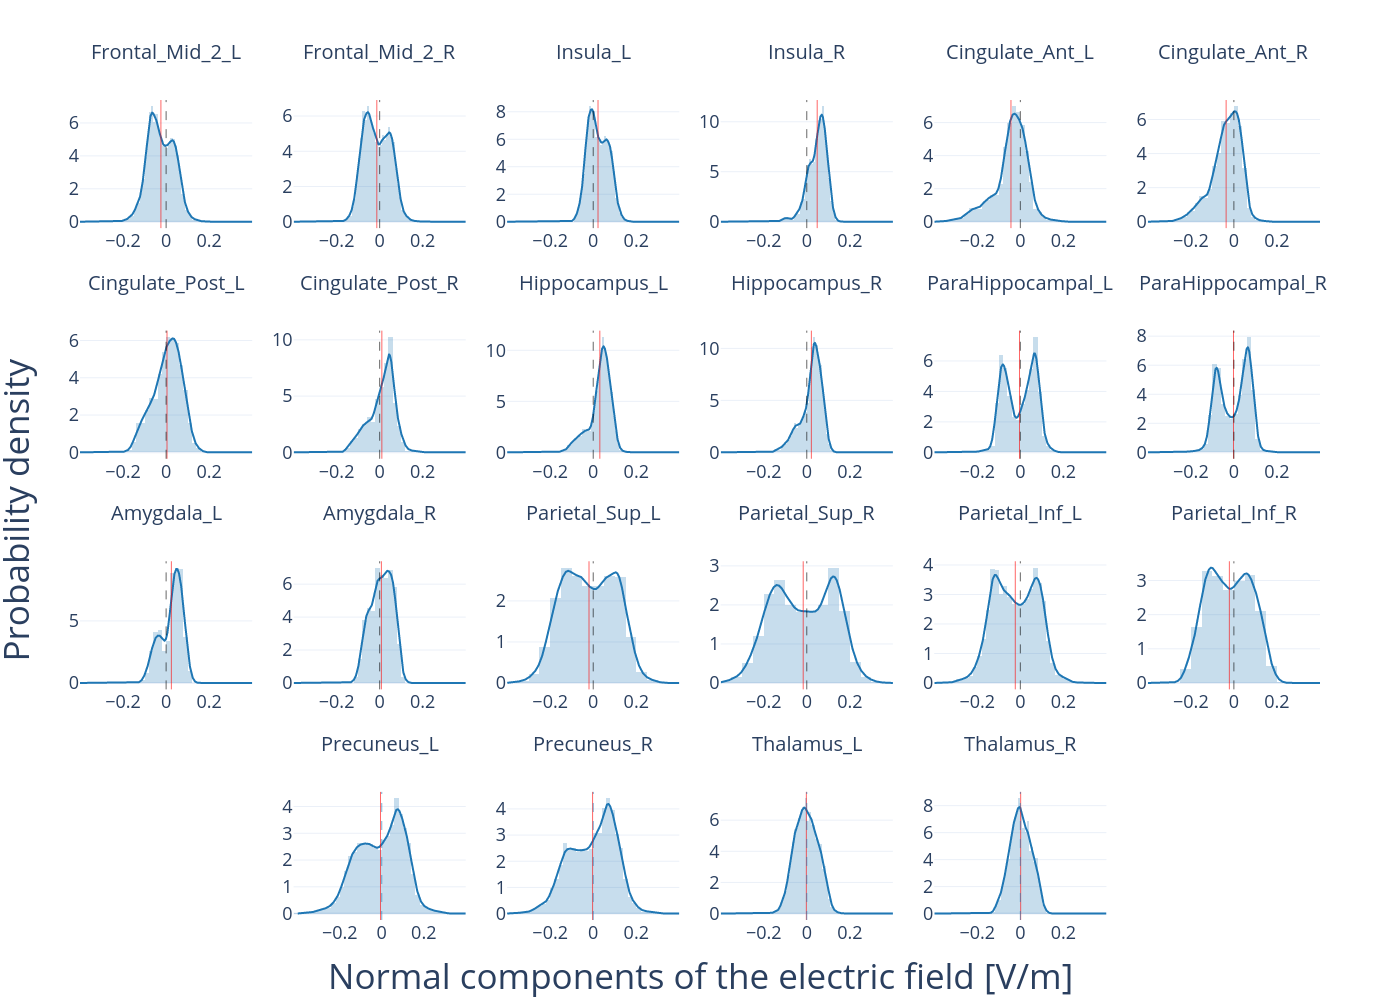
\includegraphics[width=1\textwidth]{fig/5.png}
% % \caption{Normal component distributions (i.e., $\underline{E}_{k\perp}$). Histograms showing the accumulated (across subjects) distribution of normal components - to the white matter surface - of the electric field generated by the Oz-Cz stimulation protocol over the regions of the cingulum bundle, and including all subjects in the computational sample.}
% %\label{fig5}
% %\end{figure}

% Regions situated along the antero-posterior axis, which are aligned with the orientation of the electric field such as the cingulate cortex, insula, and middle frontal gyrus, showed distributions that tended to be unimodal with a slight skewness, shifting the mean towards either positive or negative values. We found that the level of gyrification was related to the strength of the bimodality observed. For instance, the cingulate cortex, which is defined in the interhemispheric face of the brain, displayed less bimodality than the middle frontal gyrus which tends to have a more intricate shape. Interestingly, all these regions exhibited a bias towards the same value in both hemispheres. For instance, both left and right insulas were positively skewed, anterior cingulate cortices were negatively skewed, and both middle frontal gyri were negatively skewed. 

% Bimodal distributions were observed in posterior regions such as the parietal cortices and the precuneus, where the intricacy of the gyrification is maximized. These parietal regions have highly symmetric distributions around zero with two strong peaks, one positive and another negative. This implies that the gyri of these regions are mostly defined perpendicular to the orientation of the electric field. Therefore, it could be expected that by stimulating with the Oz-Cz protocol, certain cells in these regions get hyperpolarized, while others get depolarized. Although some studies \citep{aberra2020simulation} have started to unravel the contradictory effects that an electric field might deliver to the pyramidal cells into a gyrus, it is yet unknown how these regions would interact with others inside a network. 

\subsubsection{The distribution of normal field components modulates the effects of the stimulation}
First, we analysed the effect of tACS on an isolated node of our model, which consists of a balanced neural network of 100 neurons with an emergent oscillatory frequency of approximately 10 Hz.
Due to the variability in the shapes of the distributions of the normal components of the electric field (Figure \ref{fig:fig1}), we decided to explore the behavior of an isolated node over the effect of the stimulation whose amplitudes are given by different prototypical distributions which summarize this observed diversity.
In this way, we considered a symmetric bimodal, and asymmetric bimodal and a gaussian distributions with zero mean and the correspondent positive-shifted version in order to have $0.1$ mean. 
The results are summarized in Figure \ref{fig:fig6}, which shows how the oscillatory frequency and the spectral power of the LFP at that frequency change depending on the external stimulation frequency and the stimulation intensity, the two variables that conform the space parameter.
Regarding the external stimulation with zero-mean probability densities, we did not observe the typical 1:1 synchronization state between external modulation and network oscillation \citep{MONTOYA20133124,PhysRevE.60.2086,PhysRevE.77.056203}.
However, for a certain value of stimulation intensity (which depends on the external modulation frequency), a 2:1 synchronization state emerged.
In this state, the system is in a regime in which the external dynamics (external modulation) is more intense than the internal dynamics (network connectivity), and therefore the former dominates over the latter.
In this region of the parameter space, we can describe the dynamics of the network
\begin{figure}[!htb]
    \centering
    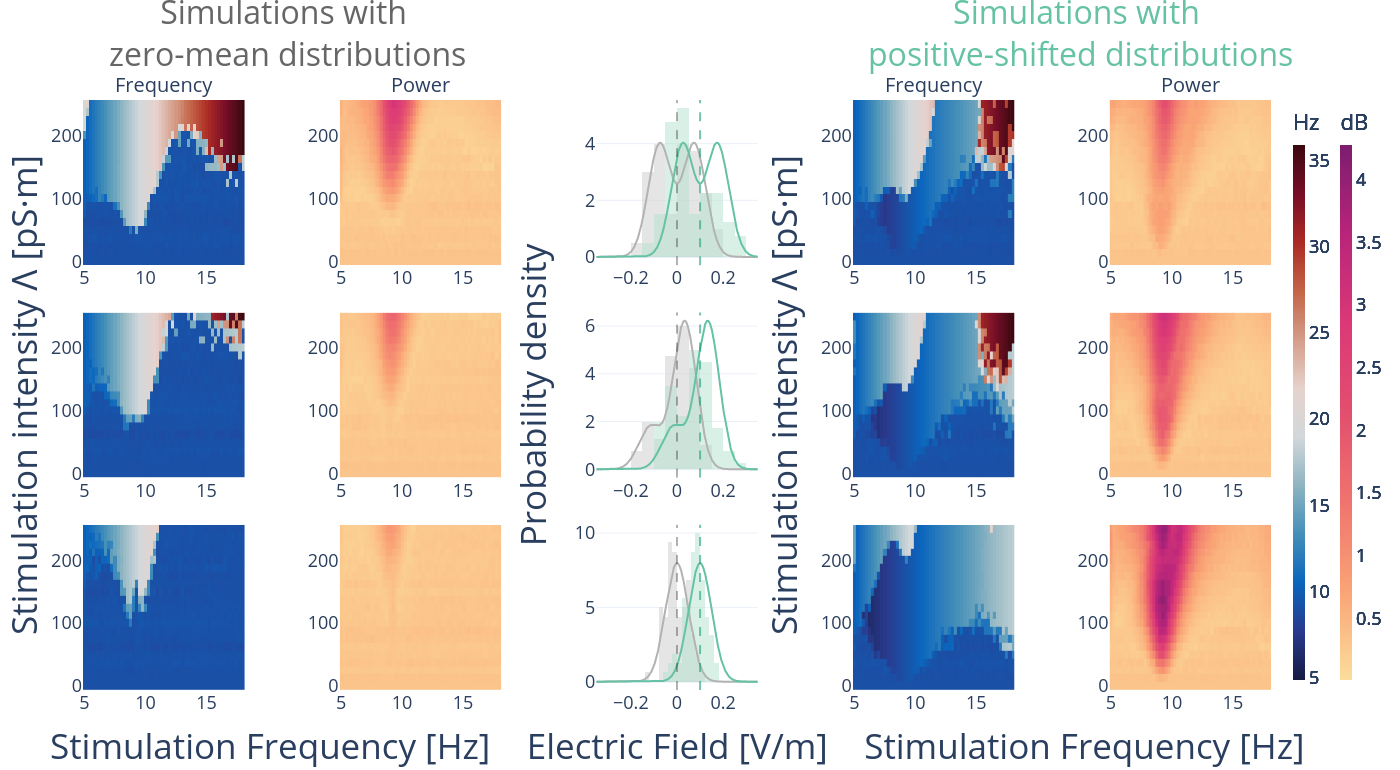
\includegraphics[width=\textwidth]{chapter3/figures/theoretical_distributions_effect.png}
    \caption{\textbf{Effects of the external stimulation on an isolated population network.}
    Oscillation frequency and power of the network are shown as functions of external modulation frequency and stimulation density for three different prototypical distributions, along with their respective positive-shifted versions.
    The distributions are presented from top to bottom: symmetric bimodal, asymmetric bimodal, and Gaussian.}
    \label{fig:fig6}
\end{figure}
as two independent dynamics each one associated to an \text{independent} sub-network. 
The neurons of one of the subnetworks receive an external stimulation with a positive amplitude, while the neurons of the other receive a stimulation with a negative amplitude.
This leads to an anti-phase dynamic between these two sub-networks, as illustrated in Figure \ref{fig:fig7} (left column), where spike histograms of the neurons during the cycle corresponding to the frequency of external modulation are depicted.
The distributions exhibit two peaks of similar amplitude at different times, whose difference in terms of phase is 180º (50 ms).
In this example we used the symmetric bimodal function, but the same behaviour is observed in the case of the other distributions.

When we used positive-shifted distributions for the stimulation, $1:1$ synchronization states started to emerge (Figure \ref{fig:fig6} right column).
As in the previous case, the limits of these regions depend on the type of distribution used. Furthermore, just as in the case where the distributions have a zero mean, the $2:1$ synchronization region also exists.
Unlike the previous case, it occurs for stimulation intensities higher frequencies higher than the network's own frequency.
\begin{figure}[!htb]
    \centering
    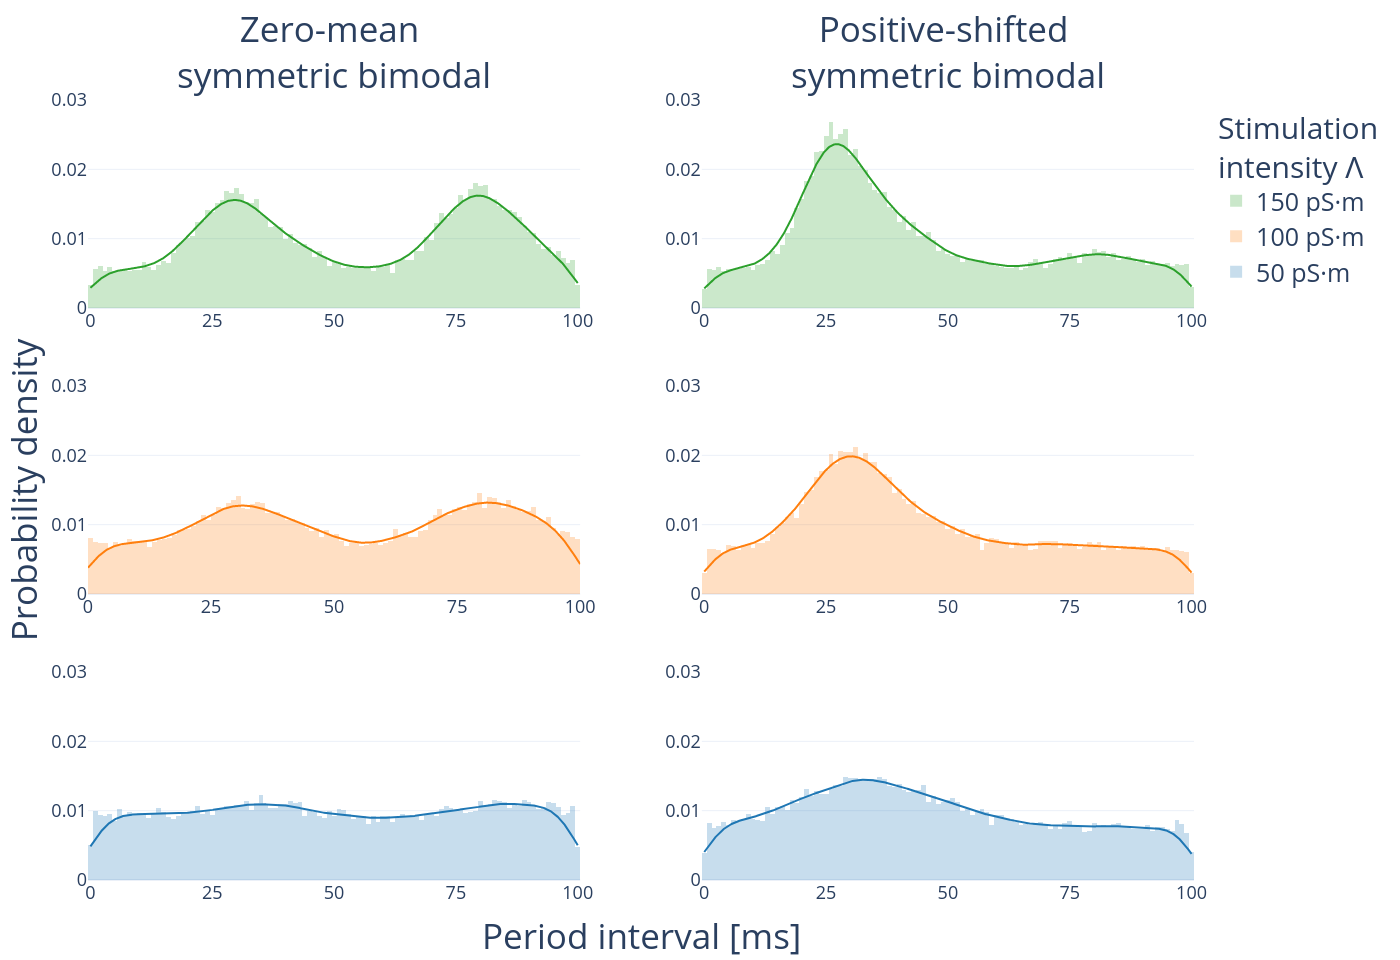
\includegraphics[width=\textwidth]{chapter3/figures/histograms.png}
    \caption{\textbf{Spiking distribution of an isolated population network}.
    Spike distributions or firing rates ver the cycle of external sinusoidal modulation at 10 Hz.
    Three different stimulation intensities have been applied, shown from top to bottom: 150, 100, and 50 pS$\cdot$m.}
    \label{fig:fig7}
\end{figure}
Similarly, the intensity value depends on the external modulation frequency.

Figure \ref{fig:fig7} (right column) shows the spike distribution over the cycle of the external distribution (10 Hz).
In this case, the 1:1 synchronization stated is characterized by a unique peak in the spikes distribution.
Two examples of these are plotted with stimulation intensities of $50$ and $100$ pS$\cdot$m.
As the stimulation intensity increases, the external dynamics begin to dominate over the internal dynamics, and again, the network dynamics can be described by two \textit{independent} sub-dynamics of two sub-networks oscillating in anti-phase.
Since the distributions are positive-shifted, the two sub-network are not equal in the number of neurons implying the emergence of two peaks with different amplitudes in the spikes histograms (Figure \ref{fig:fig7}, right column, stimulation intensity = $150$ pS$\cdot$m).

The response of the network to this stimulation is similar (especially in the case of shifted distributions) for both types of bimodal stimulation.
However, when we look at the spectral power, a greater increase in power is achieved when using a Gaussian distribution, followed by the asymmetric bimodal distribution, and finally the symmetric bimodal distribution (Figure \ref{fig:fig6}, right column).

Therefore, we can qualitatively determine that the shape of the distribution plays an important role, as well as the mean of that distribution.
On the one hand, a higher mean in absolute value allows the appearance of the expected 1:1 synchronization states.
On the other hand, the shape of the distribution will determine a greater or lesser increase in spectral power at the frequency of interest, which in our case is the network's own frequency.

\subsection{Working-point determination in the data-driven cingulum bundle network model}
We have designed a personalized resting-state spiking neural model that represents the cingulum bundle.
This personalization remains in the data extracted experimentally that drives the model: the connectivity matrix, given by the number of tracts between regions, and the delay matrix, computed by the length of those tracts.
Therefore, what we have designed is a scheme that,  given this two matrices, we can design a model that would represent the brain network associated with a given subject.

However, to fine-tune the personalized model, we have to determine the so-called \textbf{working point}.
It determines the optimal point of parallelism between the dynamics of the model and the subject's brain.
To do this, it is common to find the parameters that optimize the correlation (usually Pearson's correlation) between the functional connectivity matrices relative to the patient and the potential model.
\begin{figure}[htbp]
    \centering
    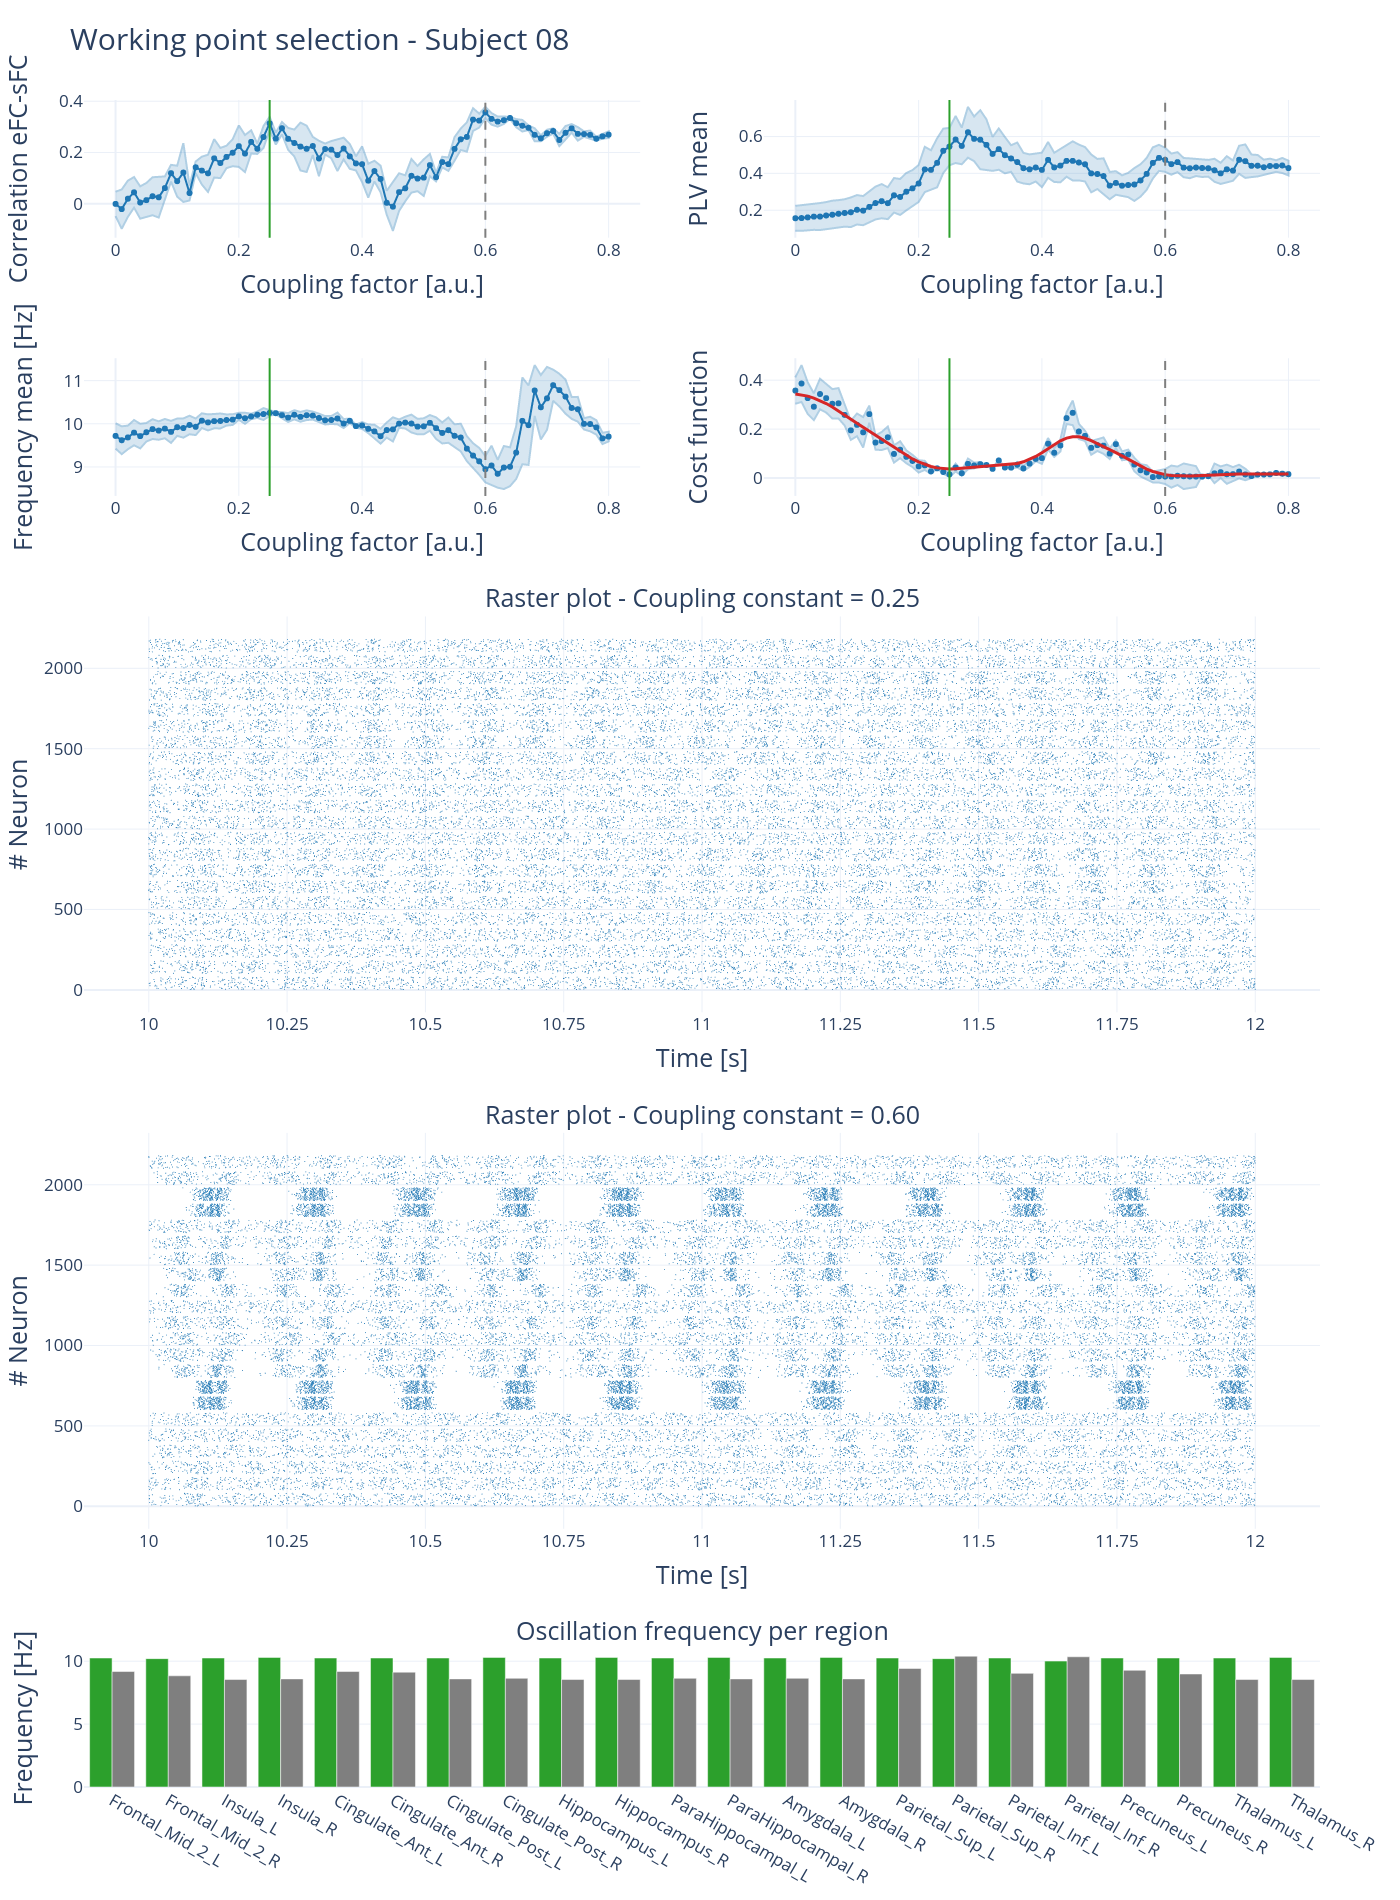
\includegraphics[width=0.9\textwidth]{chapter3/figures/working-point.png}
    \caption{\textbf{Selection of the working point in the network related to subject 08}.
    The initial four panels depict the variables used to compute the coupling factor: correlation between experimental and simulated functional connectivity, average PLV mean, and average frequency across network regions.
    A Gaussian smooth fit (red curve) aids in identifying the minima in the cost function plot, with the green line indicating the working point and the gray dashed line representing the working point obtained through correlation maximization.
    The subsequent two plots compare the raster plots of the entire network at the two working points, while the bottom plot illustrates the frequency oscillation of each ROI for these coupling factor values.}
    \label{fig:working-point-determination}
\end{figure}
In our case, we determine the coupling factor, which is a constant that multiplies the connectivity matrix and determines the final value of the conductances of the synapses between regions.
In previous works, propagation velocity was also considered as another parameter to be optimized in the working point determination procedure \citep{cabral_role_2011,nakagawa_how_2014}.
However, we set this parameter fixed at 15 m/s, which is and appropriate value and other studies have considered similar value \citep{cabrera-alvarez_modeling_2023}, and, previously, we observed that it was not too determinant in the optimization of the working point.

Initially, this method provided us non-satisfactory results, and therefore, we added additional conditions.
On the one hand, that the average oscillation frequency among all regions was as close as possible to 10 Hz, and on the other hand, that the mean functional connectivity matrix of each region (mean of the PLV matrix) was as close as possible to 0.45.
This last condition was proposed to make the functional connectivity matrix more realistic in comparison with experimental ones.
Therefore, there are three variables to consider in the definition of our \textbf{cost function} to determine the working point of the model for each subject: maximizing the \textbf{correlation} between experimental and theoretical functional connectivity ($r$), having the \textbf{average oscillation frequency} ($\langle f \rangle$) as close as possible to 10 Hz, and having the \textbf{average phase locking value} ($\langle PLV \rangle$) as close as possible to 0.45.

For some subjects, minimizing the cost function resulted in a coupling factor value where some regions exhibited high activity and high synchronization states with a lower oscillation frequency.
Therefore, an additional criterion was considered for the first relative minimum of the cost function.
An example of this scenario is shown in Figure \ref{fig:working-point-determination}, which shows the three variables to consider, the cost function, the raster plots of relatives to the network at the working point and the coupling factor value that minimizes the cost function, and the oscillation frequency value of all regions between these two points (the corresponding plots for the other subjects are placed in Appendix B Figures \ref{a-fig:working_point_subject_1} - \ref{a-fig:working_point_subject_10}).
This example illustrates how the choose of the coupling factor value that maximizes the correlation produces undesirable dynamical states.
A coupling factor = 0.6, for some regions, is strong enough to exhibit a well defined oscillation with a high synchronization among their neurons.
Furthermore, this oscillation results in a reduction to the target of 10 Hz, specifically around 8 Hz, in the majority of the cases.
Those regions with this oscillation mode are those that are more intensively connected to others.
The raster plot of the network in the working point exhibits a desirable noisy dynamic, with all nodes oscillating at a similar frequency in a similar synchronization state.
\begin{table}[!htb]
 \caption{Comparison of the working point results between our criteria and the criterion of only considering the correlation between the experimental and computational functional connectivities.
 The rightmost column indicates the performance of the correlation criteria: red indicates undesired dynamics, orange represents a limit situation nearing high activation and synchronization state, and green indicates equivalent or better results compared to our criteria.}
    \def\arraystretch{1.3}%  1 is the default, change whatever you need
    \centering
    \begin{tabular}{|c||c|c|c|c||c|c|c|c||c|}
        \hline
         & \multicolumn{4}{c||}{Our criteria} & \multicolumn{4}{c||}{Correlation} & 
         \multirow{2}{5mm}{} \\
         \cline{2-9}
         \cline{2-9}
         & $c $&  $r$ & $\langle PLV \rangle$ & $\langle f \rangle$ & $c$ &$r$ & $\langle PLV \rangle$ & $\langle f \rangle$ & \\
         \hline
        Subject 01  & 0.33 &	0.62  & 0.50 & 9.84  & 0.74 & 0.63 & 0.61 & 10.74 &  \cellcolor{red} \\
        \hline
        Subject 02  & 0.30 &	0.21  & 0.50 & 10.16 & 0.25 & 0.23 & 0.48 & 10.15 & \cellcolor{green}\\
        \hline
        Subject 03  & 0.28 & 0.13  & 0.74 & 10.11 & 0.39 & 0.23 & 0.66 &  9.77 & \cellcolor{orange}\\
        \hline
        Subject 04  & 0.55 &	0.29  & 0.44 & 9.99  & 0.52	& 0.33 & 0.55 &  10.01 & \cellcolor{green}\\
        \hline
        Subject 05  & 0.20 & 0.36  & 0.53 & 10.17 & 0.30	& 0.74 & 0.55 &	 10.10 & \cellcolor{green}\\
        \hline
        Subject 06  & 0.35 & 0.17  & 0.39 & 10.07 & 0.44	& 0.26 & 0.55 & 10.42 & \cellcolor{orange}\\
        \hline
        Subject 07  & 0.35 & 0.34  & 0.34 & 10.17 & 0.62	& 0.72 & 0.47 & 10.24 & \cellcolor{red}\\
        \hline
        Subject 08  & 0.25 & 0.31  & 0.55 & 10.25 & 0.60 & 0.36 & 0.47 & 8.95 & \cellcolor{red} \\
        \hline
        Subject 09  & 0.30 & -0.08 &	0.43 & 10.19 & 0.73	& 0.16 & 0.52 & 9.83 & \cellcolor{red} \\
        \hline
        Subject 10 & 0.42 & 0.10  & 0.44 & 9.92 & 0.59 & 0.11 & 0.54 & 9.54 & \cellcolor{red} \\ 
        \hline
    \end{tabular}
    \label{tab:working-point}
\end{table}

\subsubsection{Comparison between different criteria}
Table \ref{tab:working-point} provides an overview of the working points for each subject's model based on our criteria, compared to those determined solely by maximizing the correlation between experimental and computational functional connectivity.
Most right column indicates if the latter method provides a good solution or not.
The red color indicates that the network at that working point exhibits a high level of synchronization, such as the one depicted in Figure \ref{fig:fig6}.
Orange color indicate intermediate situation, where the dynamics is at the limit of the emergence of high synchronization state.
Green color indicates those cases in which both method are equivalent or even better.

While, considering only correlation, we obtained bad results in five different subjects and other two being in the limit before the undesired dynamics emerges.
For only three subjects the method was good enough.
Therefore, the addition of other variables was necessary with the reduction of correlation between the functional connectivity matrices.

\subsection{Properties of resting-state dynamics.}
The dynamics of the neural networks exhibit diverse dynamics: while certain regions remain minimally synchronized over time, others undergo fluctuations between states of high synchronization and periods of lower synchrony \citep{battaglia_temporal_2007,lachaux1999measuring,doi:10.1089/brain.2015.0362}.
Figure \ref{fig:plv_dynamics} illustrates the functioal connectivity in different time intervals exhibiting such fluctuations.
\begin{figure}[htbp]
    \centering
    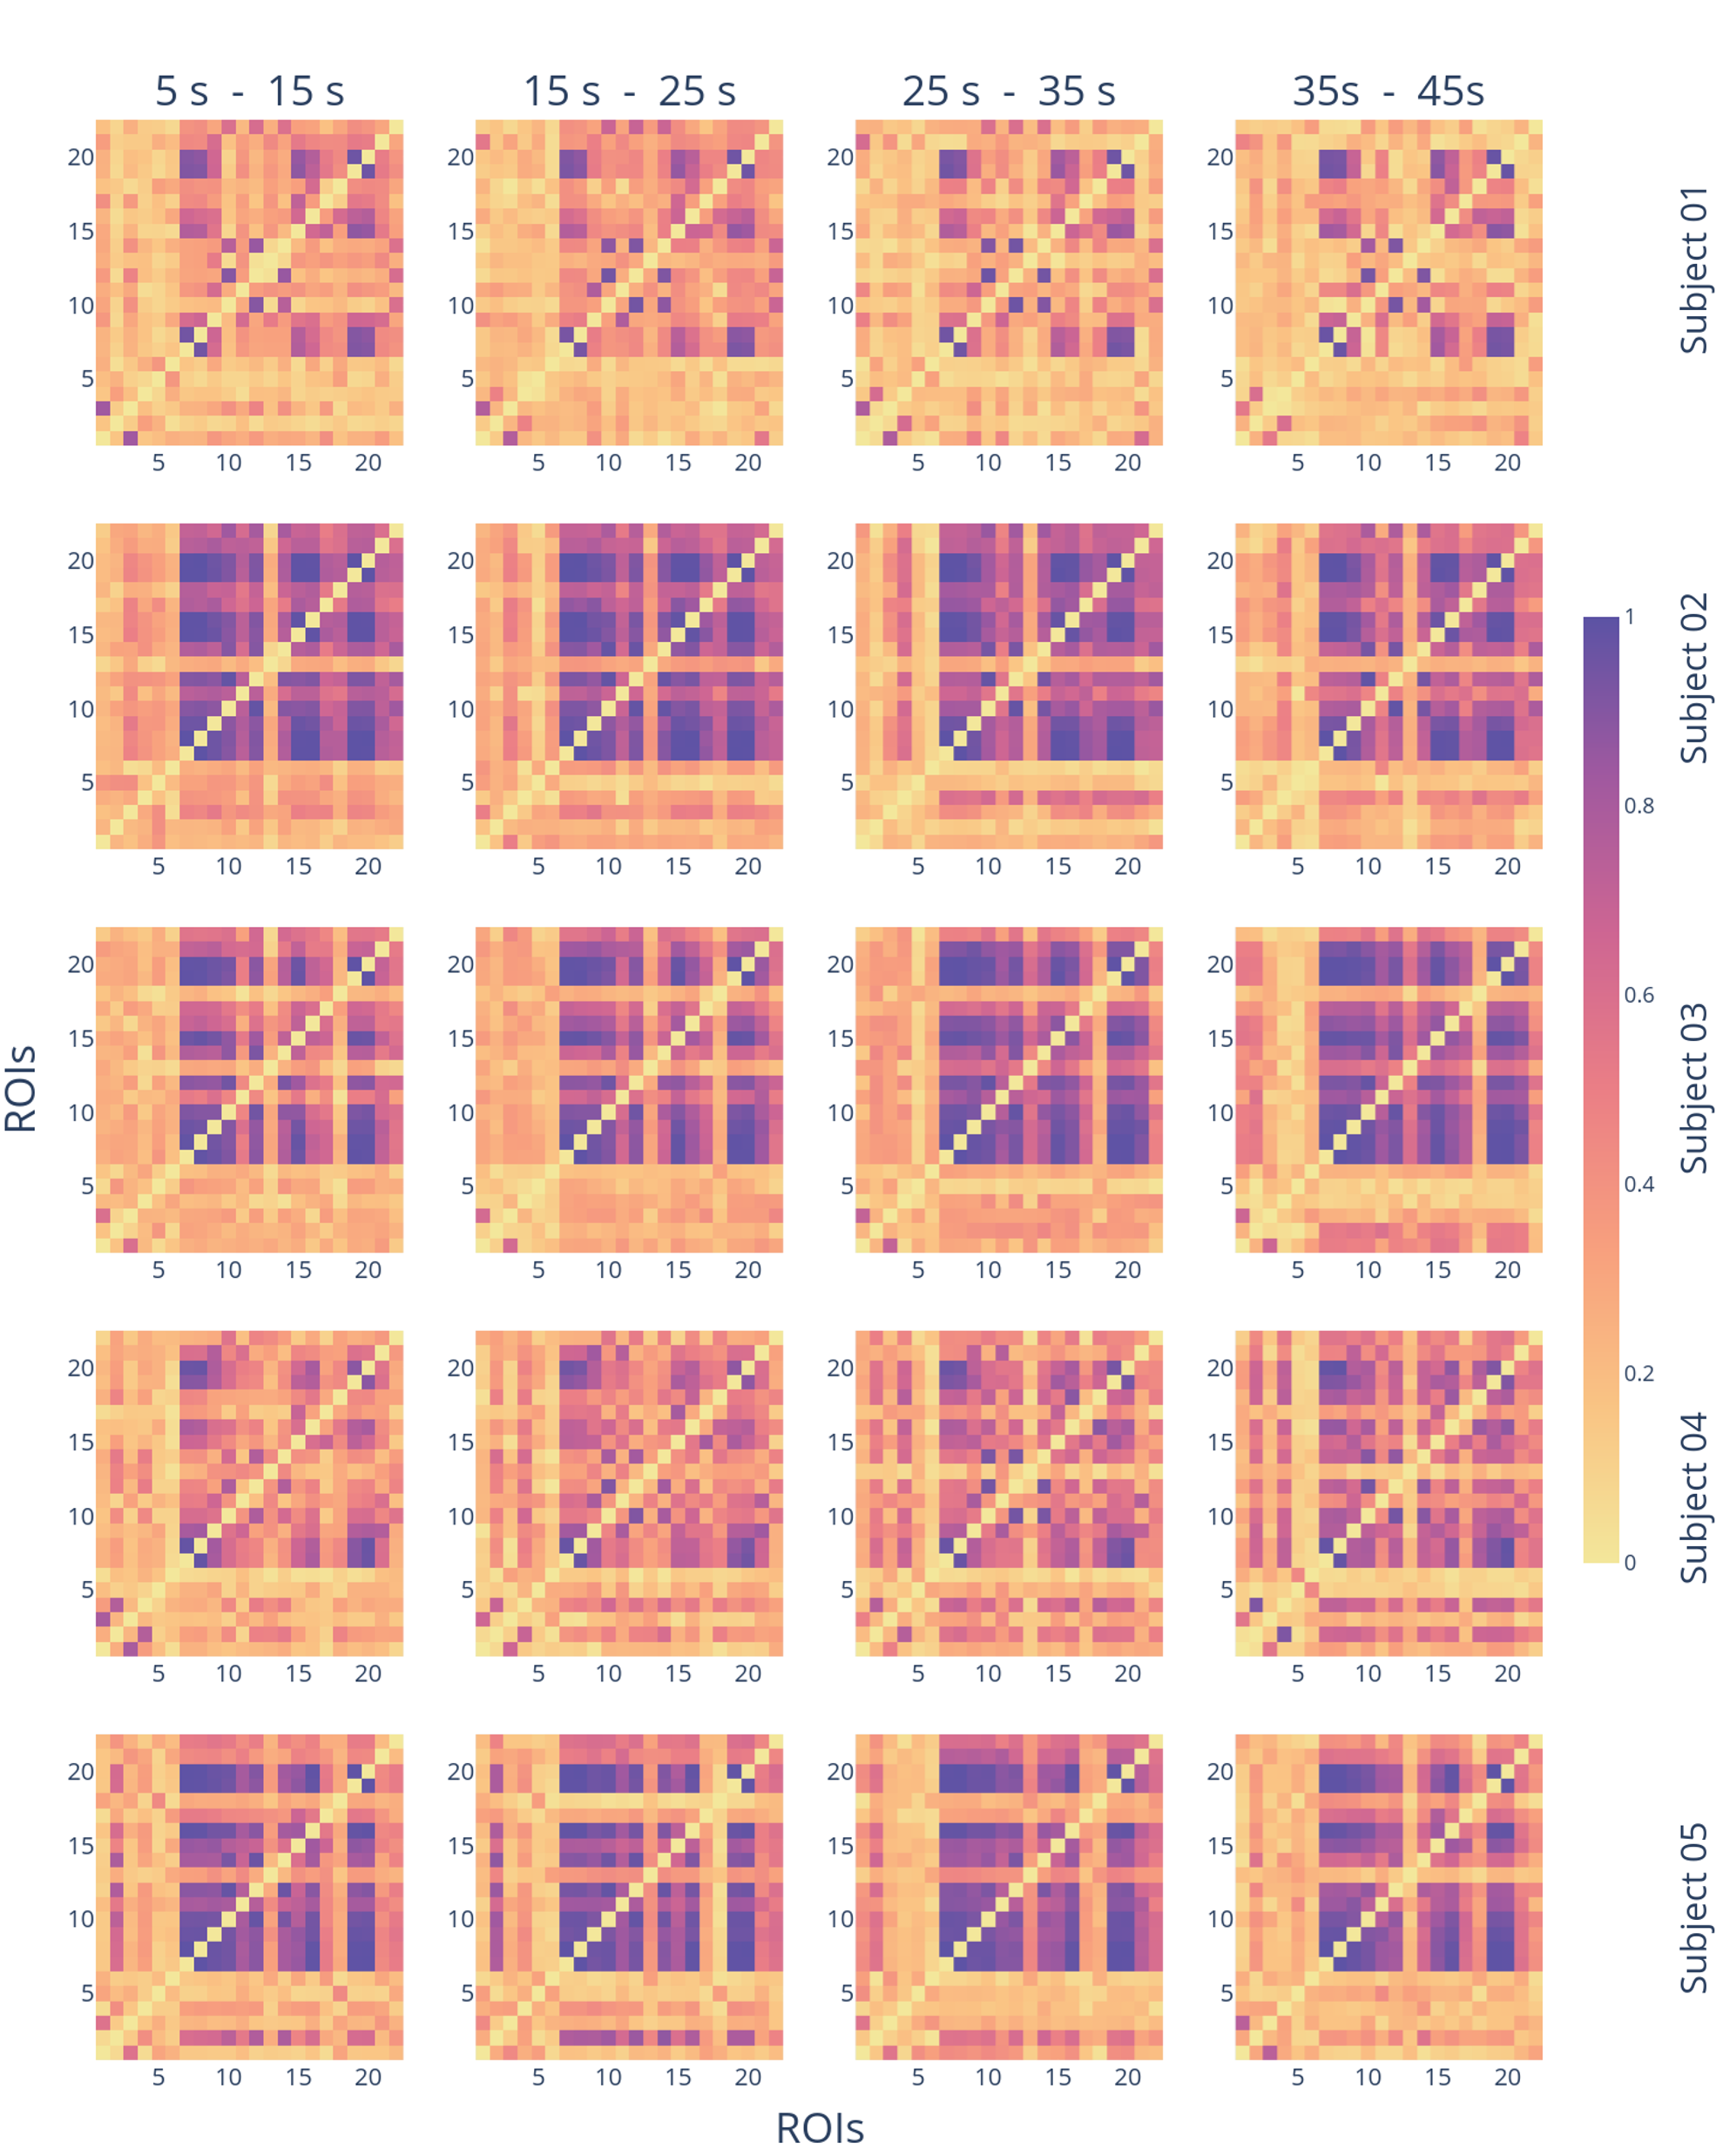
\includegraphics[width=\textwidth]{chapter3/figures/plv_dynamics_0.png}
    \caption{\textbf{Functional connectivity matrices for different time intervals}.
    Subjects 01 - 05.}
    \label{fig:plv_dynamics}
\end{figure}
\begin{figure}[htbp]
    \ContinuedFloat % To indicate continuation of the previous table
    \centering
    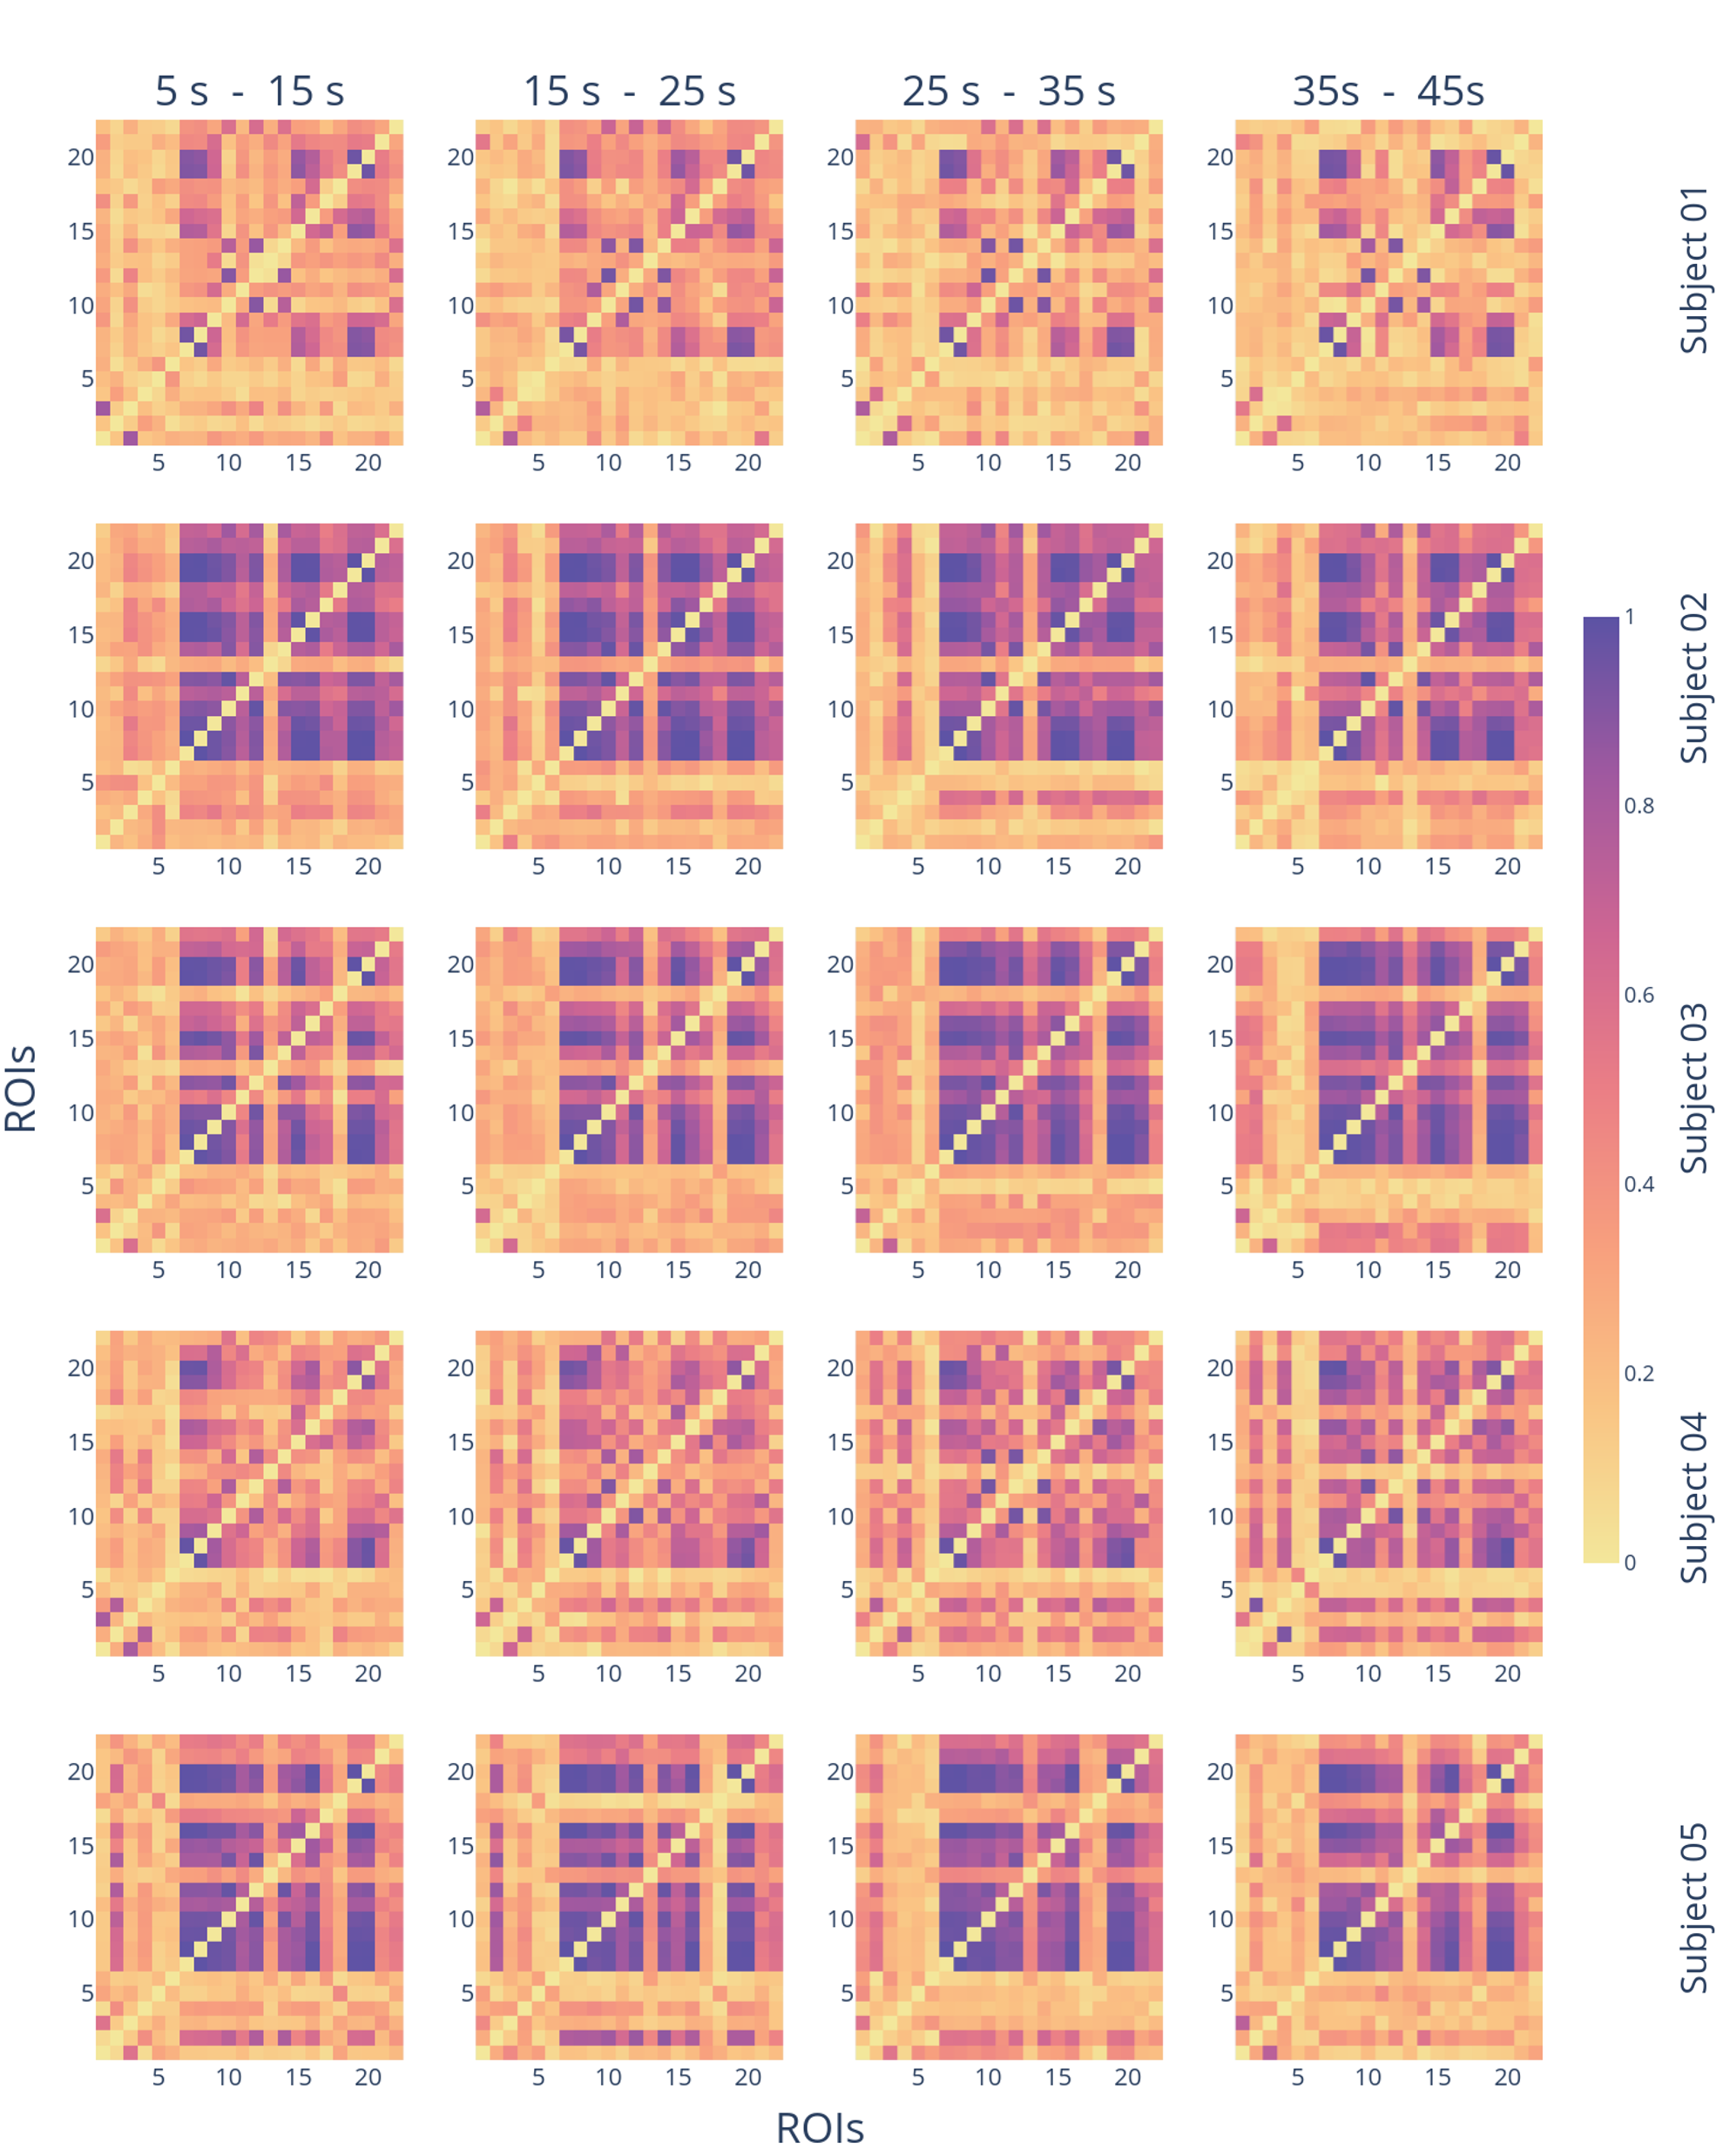
\includegraphics[width=\textwidth]{chapter3/figures/plv_dynamics_0.png}
    \caption{\textbf{Functional connectivity matrices for different time intervals (continuation)}.
    Subjects 06 - 10.}
    % \label{fig:plv_dynamics_2}
\end{figure}

\subsection{Alpha spectral power rise in the resting-state spiking network model}
We investigated the effect of tACS on our resting-state network model. 
For this purpose, we had the distributions of the normal components of the electric field for each region, obtained by the ROAST method.
In our computational design, this stimulation is carried out by assigning a field amplitude to each neuron.
In other words, each region is associated with a distribution of field components and each neuron belonging to that region is assigned a randomly generated field amplitude based on that distribution.
Therefore, for each region, the neurons experience a different influence from the electric field with opposite signs (anti-phase alternating electric fields).
\begin{figure}[htbp]
    \centering
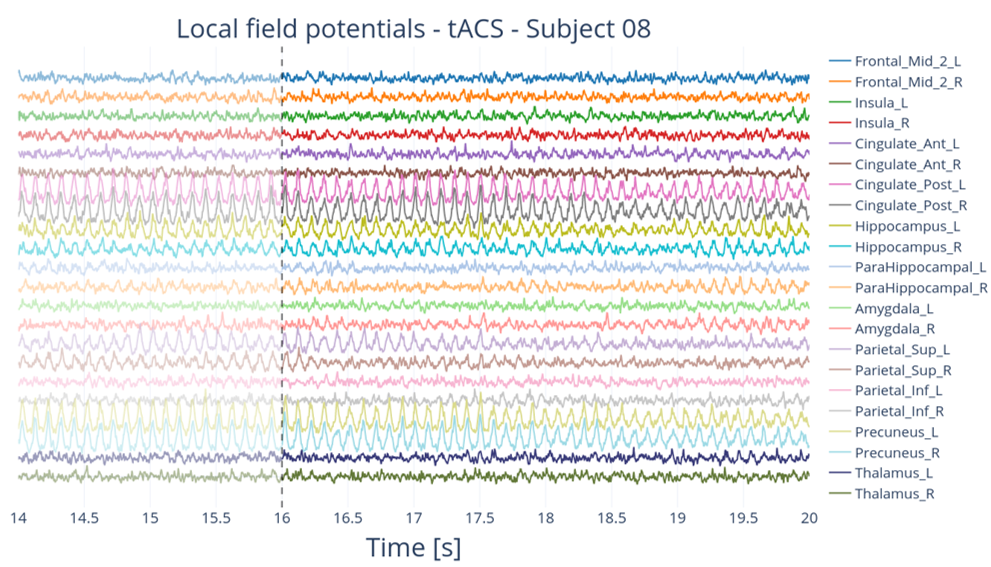
\includegraphics[width=\textwidth]{chapter3/figures/lfps_stimulation_7.png}
    \caption{\textbf{LFPs before and during tACS}.
    LFPs of each region of the model relative to subject 08 during the protocol of stimulation.}
    \label{fig:stimulation-output}
\end{figure}
This protocol differs from the conventional protocol, where computationally, a common field amplitude is considered for all neurons within the same region, usually the average of the distributions \citep{merlet_oscillatory_2013}.

Our C3N collaborators performed tACS experiments in healthy patients, different from those whose data we used for the design of our models, and detected an increase of $\sim 8\%$ in the alpha peak between subjects \citep{cabrera-alvarez_understanding_2023}.
This procedure was similar to the one reported in the previous study, where a 14\% was achieved \citep{zaehle_transcranial_2010}.
This measurement was not computed by averaging the effect of all regions of the network.
In the experiments, our collaborators applied a cluster-based permutation test to detect those areas whose alpha power was increased after the stimulation.
Therefore, in our simulations, we proceed in a similar way, by computing the alpha power change among all those areas as a whole, which consists in thirteen areas.
The regions in our model that were included in that cluster were: \textit{Frontal\_Mid\_2\_L}, \textit{Insula\_L}, \textit{Insula\_R}, \textit{Cingulate\_Ant\_L}, \textit{Cingulate\_Ant\_R}, \textit{Hippocampus\_L}, \textit{Hippocampus\_R}, \textit{ParaHippocampal\_L}, \textit{ParaHippocampal\_R}, \textit{Amygdala\_L}, \textit{Parietal\_Sup\_R}, \textit{Parietal\_Inf\_R} and \textit{Precuneus\_R}.
Therefore, similarly to the experiments, we measured the effects in the alpha band considering these regions as whole.

The stimulation frequency for each personalized model is determined by the average frequency of the regions within the cluster in the resting state.
On the other hand, we have a free parameter in the stimulation, which is its intensity.
This parameter determines the effective amplitude of the stimulation and is identical for all neurons in the network, as described in equation \eqref{eq:tacs}.
In our computational experiment, tACS was administered for a duration of 34 seconds, preceded by 16 seconds of resting-state dynamics.
Figure \ref{fig:stimulation-output} illustrates the LFP signals from all regions of the model for subject 08 during both resting state and stimulation.
Additional LFP data for the remaining subjects are shown in Appendix B Figures \ref{a-fig:stimulation-output-1} - \ref{a-fig:stimulation-output-10}.

Figure \ref{fig:alpha-rise-cluster} illustrates the observed increase in alpha spectral power between subjects, resulting in an average increase of $8\%$.
However, when considering each personalized network model individually, we found that the alpha power only increased in four subjects: 01, 04, 07, and 10.
In contrast, in subjects 02, 05, and 06, the power decreased, while subjects 08 and 09 did not show any noticeable effect.
\begin{figure}[htbp]
    \centering
    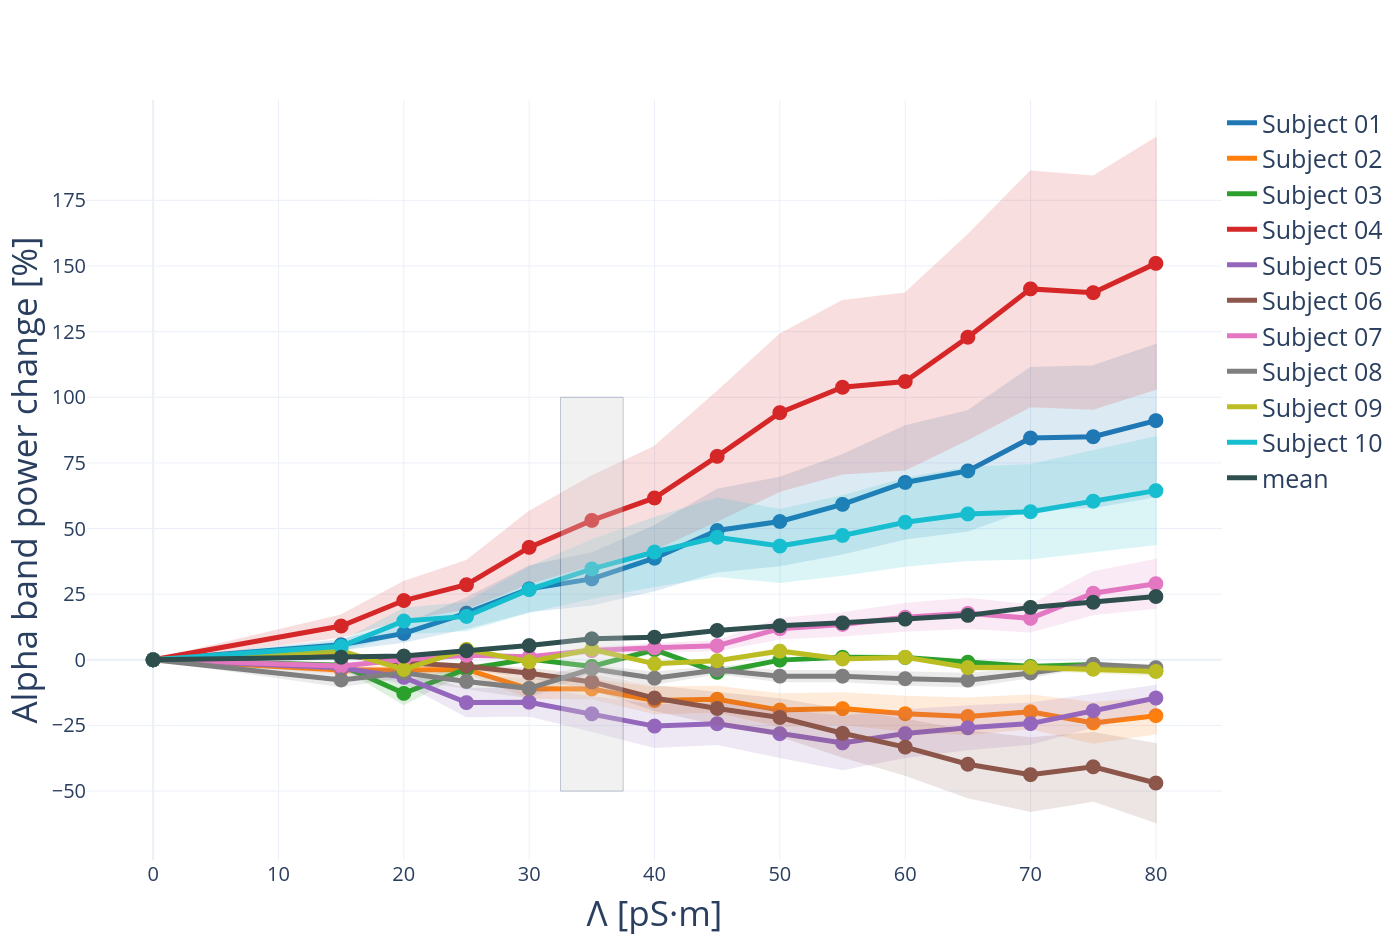
\includegraphics[width=\textwidth]{chapter3/figures/alpha_rise_cluster.png}
    \caption{\textbf{Alpha spectral power rise across subjects}.
    Each line represents the effect of the alpha band power over the regions belonging to the cluster
    as a function of the intensity of the external stimulation.
    Shadowed areas represent the standard deviation computed by 10 different realizations}
    \label{fig:alpha-rise-cluster}
\end{figure}
\clearpage 

\subsection{The mean of the distributions is a major indicator of alpha increase}
We conducted a stepwise multiple linear regression (MLR) analysis, depicted in Figure \ref{fig:MLR}, to assess the influence of the different variables that may influence the increase in alpha power within the regions: the \textbf{absolute value of the mean}, the \textbf{skewenes}, the \textbf{kurtosis} and the number of \textbf{modes of the normal components} of the field distributions,
the logarithm of \textbf{structural connectivity} and the \textbf{functional connectivity} at resting-state.

Among all these factors, the coefficient linked to the mean of the normal component distribution of the electric field displayed a direct correlation with the alteration in alpha power (coefficient = 0.44, SE = 0.039, p < 0.0001).
Similarly, other variables associated with the distributions, such as \textbf{skewness} (coefficient = -0.256, SE = 0.049, p < 0.0001), \textbf{kurtosis} (coefficient = -0.137, SE = 0.053, p = 0.009), and the \textbf{number of modes} (coefficient = -0.0687, SE = 0.029, p = 0.017), exhibited statistically significant coefficients.
\begin{figure}[!htb]
\centering
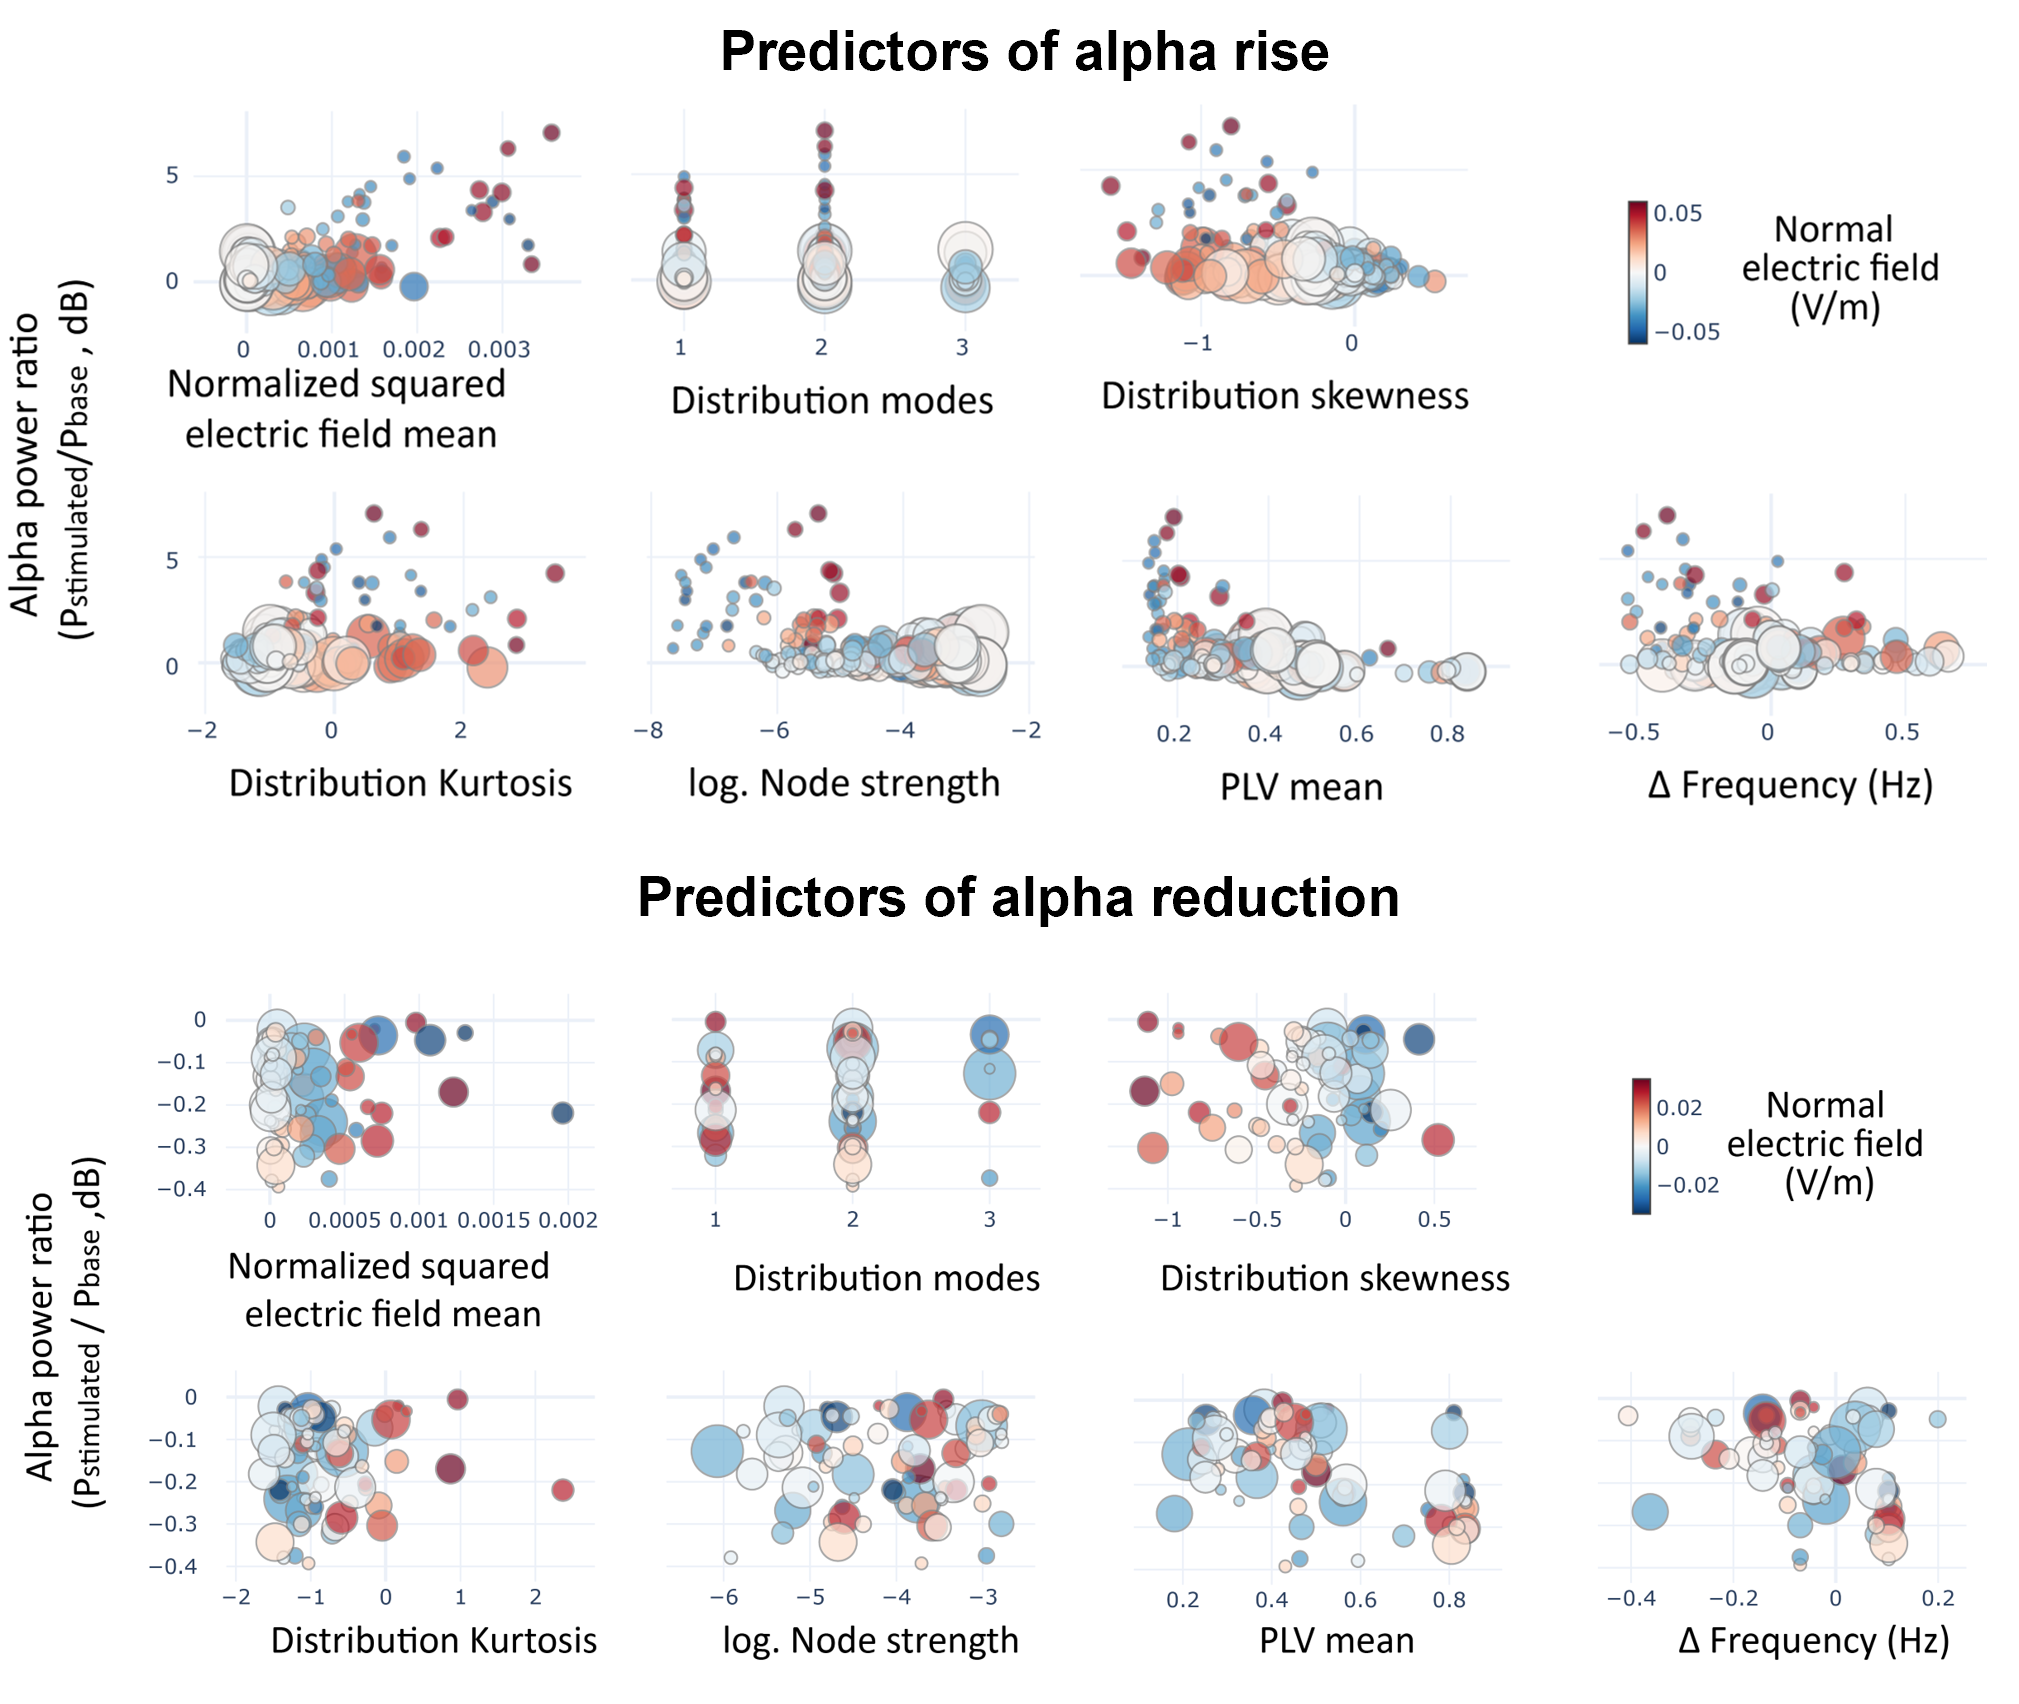
\includegraphics[width=\textwidth]{chapter3/figures/LRM.png}
 \caption{\textbf{Predictors for alpha power rising and reduction.}
 Influential factors in alpha power rising (top) and reduction (bottom) during tACS.
 The scatter plots depict the mean increase in alpha power across simulated regions that exhibited a decline compared to baseline, considering variables included in the multiple linear regression model. Point size reflects the average node strength of the region, while color denotes the normal component of the electric field. Remarkably, the sole statistically significant predictor of alpha power reduction was the mean phase locking value (PLV).
 Figure edited from \citep{cabrera-alvarez_understanding_2023}.}
\label{fig:MLR}
\end{figure}
Concerning \textbf{functional connectivity} during resting-state, it emerged as a superior predictor of alpha power augmentation (coefficient = -0.2, SE = 0.034, p < 0.0001) compared to \textbf{structural connectivity} (coefficient = -0.1, SE = 0.037, p = 0.008).

Although the absolute value of the mean proved to be the most robust predictor for the rise in alpha power, it only induced an increase in 4 out of 10 subjects.
Conversely, 4 subjects experienced a decrease in alpha power, while 2 subjects exhibited no significant alterations.
Given the relatively minor reduction in alpha power compared to the increase, we explored whether these factors directly caused a decline or mitigated the amplifying effect.
To investigate further, we constructed an additional MLR model for the data where power decreased during stimulation.
This analysis revealed that only \textbf{functional connectivity} (coefficient = -0.0423, SE = 0.007, p < 0.0001) could predict the decrease in power, whereas structural connectivity exhibited a protective influence (coefficient = 0.024, SE = 0.01, p = 0.015).
The remaining variables did not demonstrate significant associations.

\subsection{The effect of inter-regional communication}
An additional factor, not included in the MLR models, that may influence the rise/decay of the alpha power is the interregional communication through synaptic coupling.
As we have explained and analyzed in the previous chapter, communication between regions, in addition to the degree of coherence (PLV), depends on the conduction delay, determined by the length of the axon, and the frequency mismatch between the emitter and the receptor \citep{pariz_transmission_2021,sanchez-claros_information_2021}.
The interplay of these two factors may enable or disable communication pathways through regions.
\begin{figure}[!htb]
    \centering
    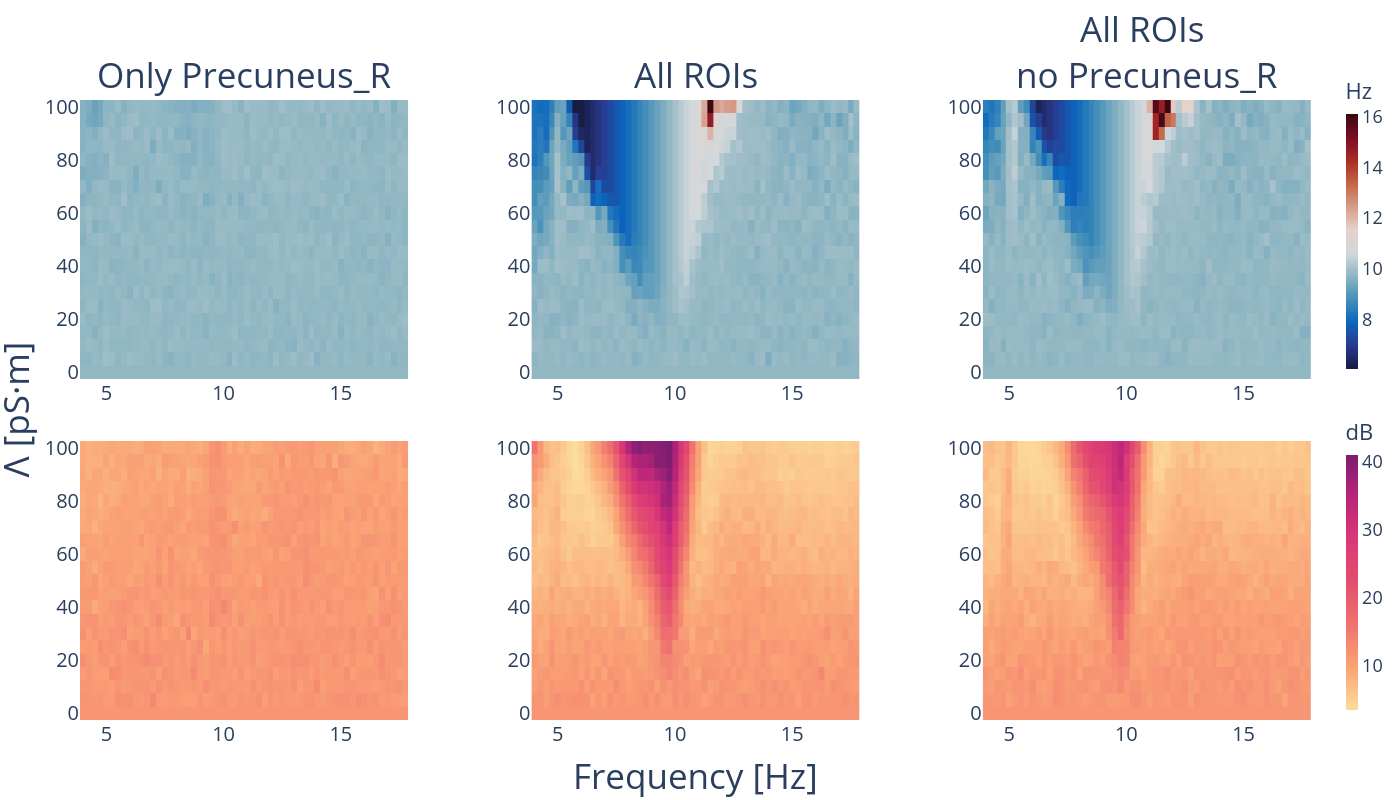
\includegraphics[width=\textwidth]{chapter3/figures/effect_of_neighboor_stimulation.png}
        \caption{\textbf{The role of inter-regional synaptic transmission in the alpha rise power}.
        Oscillation frequency and power in the \textit{Precuneus\_R} region of the network model are illustrated under three stimulation conditions: when only this region is stimulated (left), when the stimulation is applied to the entire network (center), and when the stimulation is applied to all regions except the \textit{Precuneus\_R} (right).
        This example highlights the role of inter-regional synaptic transmission in the alpha rise power, as direct stimulation alone does not yield an effect.}
    \label{fig:effect-of-interregion-stimulation}
\end{figure}
In a favorable scenario of effective communication, the power rise could be transmitted interregionally, and contribute to the power increase of connected regions.

To explore this idea, Figure \ref{fig:effect-of-interregion-stimulation} shows an example demonstrating the impact of external stimulation on a specific region as a result of transmission from interconnected regions.
In this particular case, we examined the effect of stimulation on the \textit{Precuneus\_R} region.
When the stimulation is solely applied to this region, no noticeable effect is observed.
However, when stimulation is applied to the entire network, we observe the expected behavior of increased power at the stimulation frequency and a 1:1 synchronization state in relation to the external signal.
To further validate that this effect is indeed caused by transmission across other regions, we investigated the stimulation protocol by removing the stimulation directed specifically to \textit{Precuneus\_R}.
The results were nearly identical to the previous case, confirming the significance of considering this effect in understanding the enhancement of alpha power.
Therefore, it is reasonable to infer the emergence of subnetworks with optimized inter-regional communication that would benefit alpha band power rise.
\clearpage
\end{document}
% \textcolor{blue}{Quizá esto puede desarrollarse más en la discusión o directamente comentarlo aquí.
% Estuve tanteando medidas de MI en esto, pero eso llevaría tiempo. Estuve un par de días y no conseguí nada en claro.}